\section{Birth and Death Process}

We can try and calculate an average RW duration

\begin{center}
    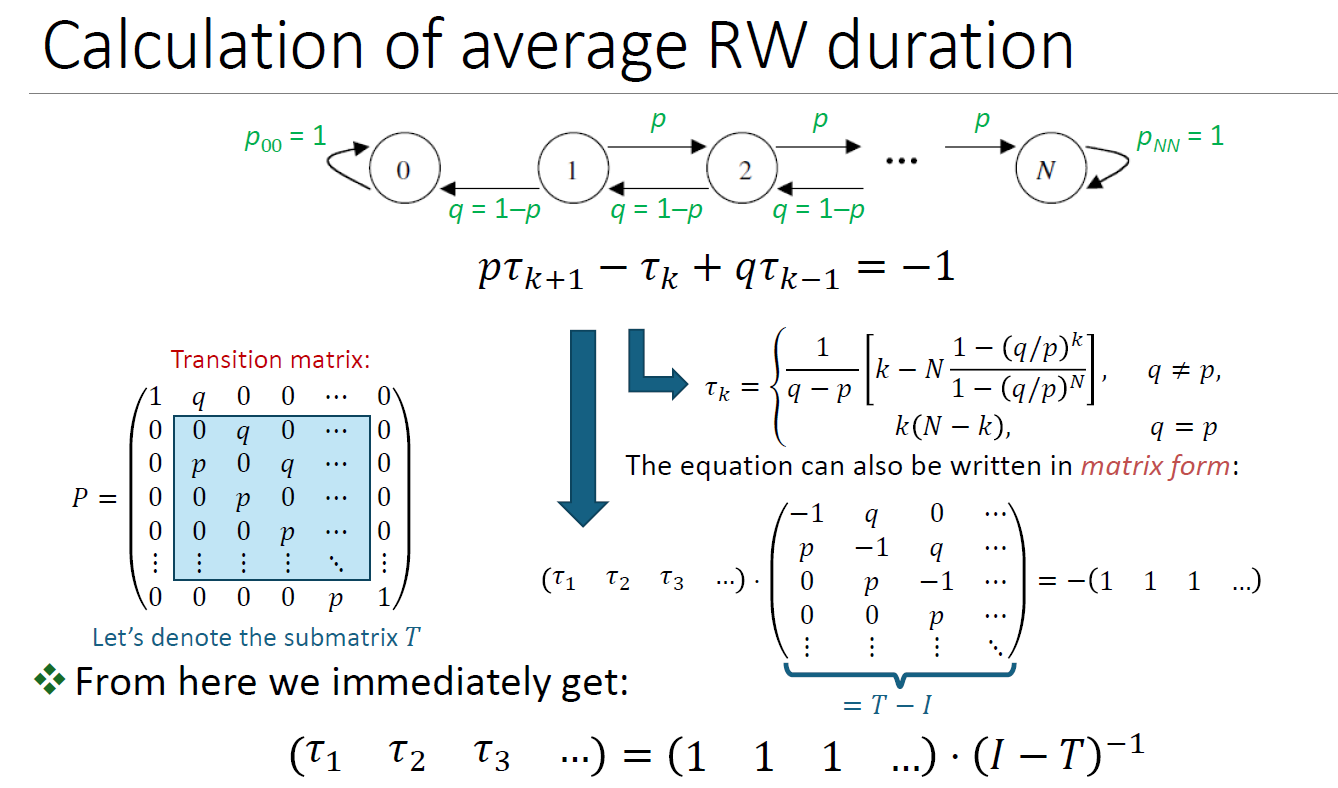
\includegraphics[width=300pt]{images/average rw duration.png}
\end{center}

If we assume that Markov chain has $k$ absorbing states. We can write its transition matrix in the following form:
\begin{equation*}
    P = \begin{bmatrix}
        I & A \\
        0 & T 
    \end{bmatrix}
\end{equation*}

where I is a diagonal $k \times k$ identity matrix, $0$ is a zero filled matrix. Define the fundamental matrix $F = (1 - T)^{-1}$ The expected times until absorbtion, if random walk starts from some particular node, can be obtained by numerically multiplying two matrices.

\begin{equation*}
    (\tau_1, \ \tau_2, \ \tau_3, \ \dots) = (1 \ 1 \ 1 \ \dots) \cdot F
\end{equation*}

\begin{center}
    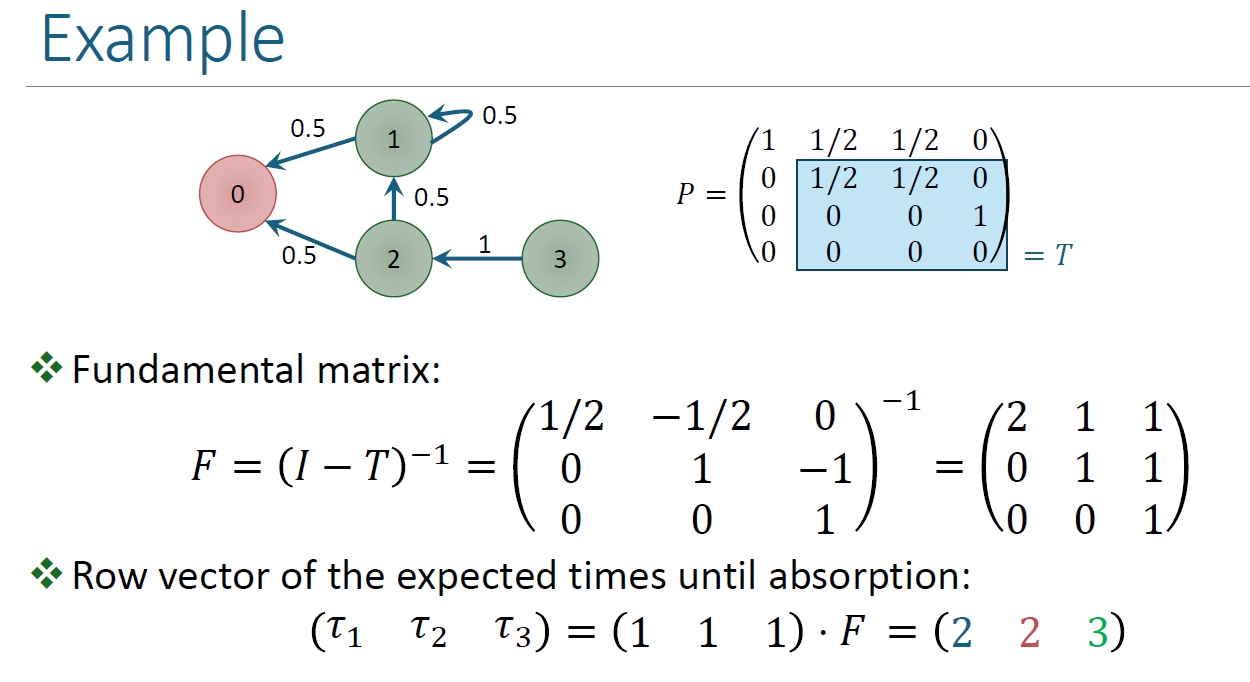
\includegraphics[width=300pt]{images/example fundamental matrix.png}
\end{center}